\documentclass{article}

% Language setting
% Replace `english' with e.g. `spanish' to change the document language
\usepackage[english]{babel}
% Set page size and margins
% Replace `letterpaper' with `a4paper' for UK/EU standard size
\usepackage[letterpaper,top=2cm,bottom=2cm,left=3cm,right=3cm,marginparwidth=1.75cm]{geometry}

% Useful packages
\usepackage{amsmath}
\usepackage{amssymb}
\usepackage{graphicx}
\usepackage{listings}
\usepackage{multirow}
\usepackage[colorlinks=true, allcolors=blue]{hyperref}
\usepackage{float}

\title{CSC446 Project\thanks{\href{https://github.com/parth2324/3D_FEM/}{Project Code Link}}}
\author{Parth Singh}

\begin{document}
\maketitle

\section{Project Description}

For the course project, I will be implementing Finite Element Method in 3D, using isoparametric quadratic elements, 
for the Laplacian PDE: $-\nabla^2u(\overrightarrow{x}) = 0$. I will be using quadratic tetrahedral Lagrange basis, and 
also discuss mesh generation under \textit{gmsh}, exploring three case studies. I will further be using Dirichlet Boundary
Condition, based on the harmonic function $g(\overrightarrow{x}) = -log(||\overrightarrow{x} - \langle -7.1, -7.2, -7.3 \rangle||)$. \\

The case studies are as follows:

\begin{enumerate}
    \item Radius 5 sphere centered at the origin (Figure \ref{fig:ex1}).
    \begin{figure}[h]
        \centering
        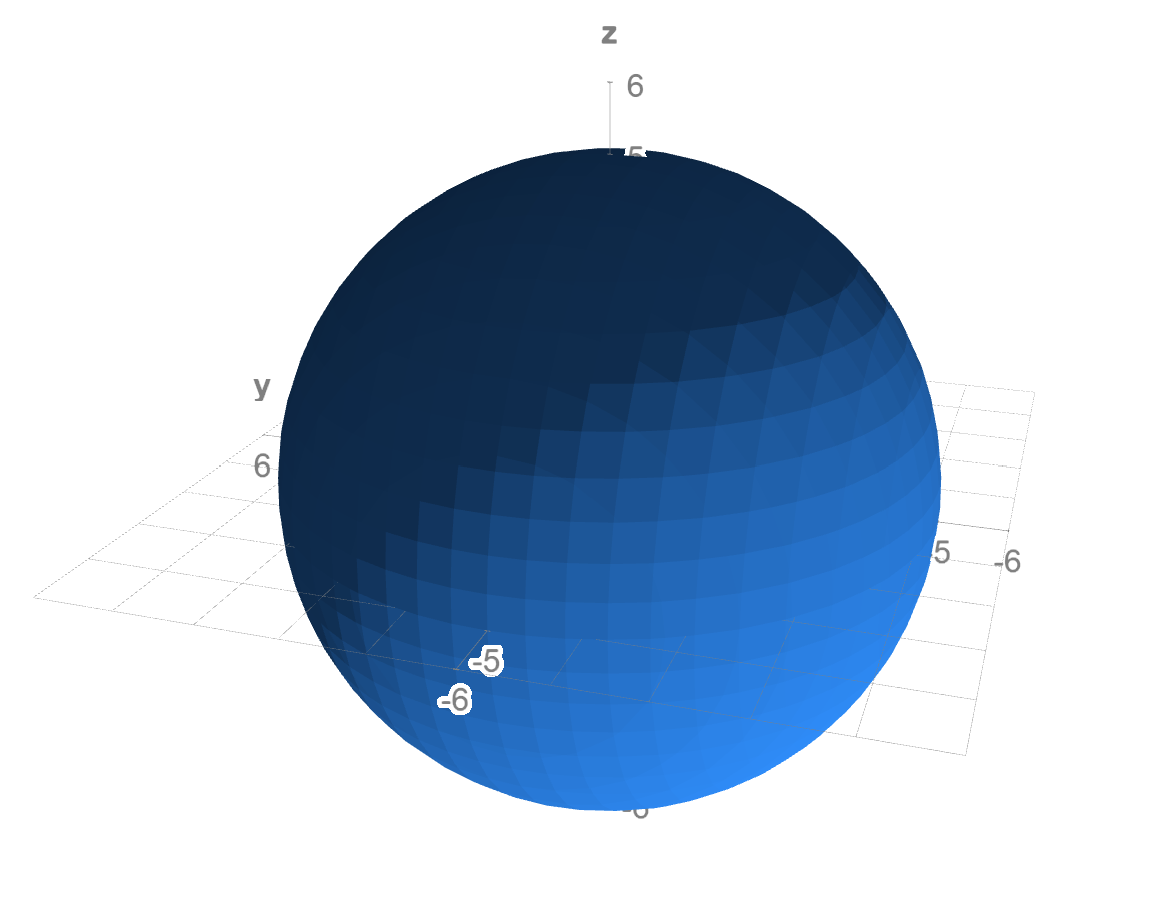
\includegraphics[scale = 0.5]{images/ex1.png}
        \caption{Radius 5 sphere.}
        \label{fig:ex1}
    \end{figure}
    \item Cylinder around the z-axis with radius 3 between $z=-5$ and $z=5$ (Figure \ref{fig:ex2}).
    \begin{figure}[h]
        \centering
        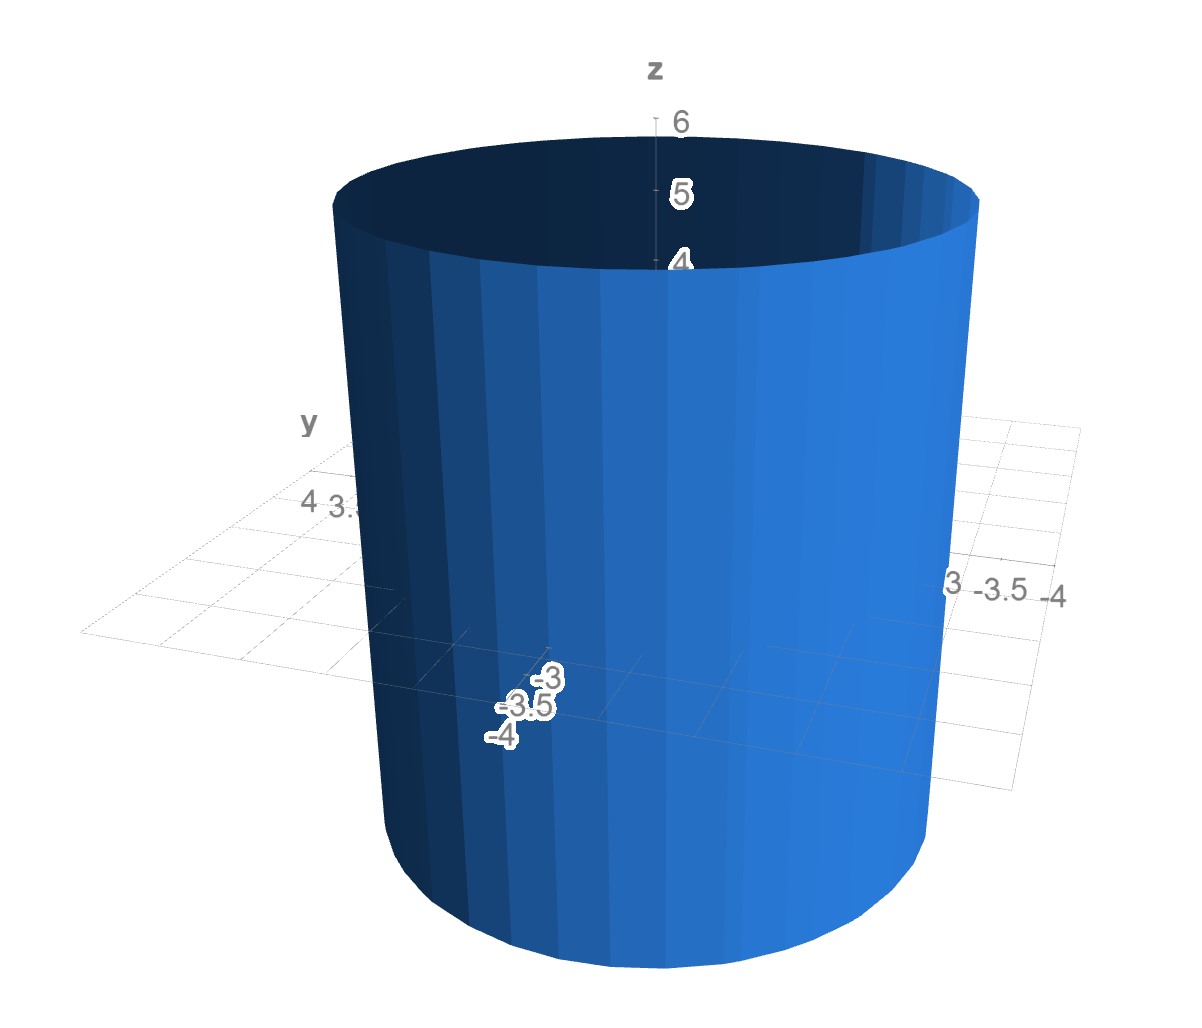
\includegraphics[scale = 0.5]{images/ex2.png}
        \caption{Radius 3 cylinder with height 10.}
        \label{fig:ex2}
    \end{figure}
    \item Cone between $z=0$ and $z=1$ with apex at origin and internal angle $5^\circ$ (Figure \ref{fig:ex3}).
    \begin{figure}[h]
        \centering
        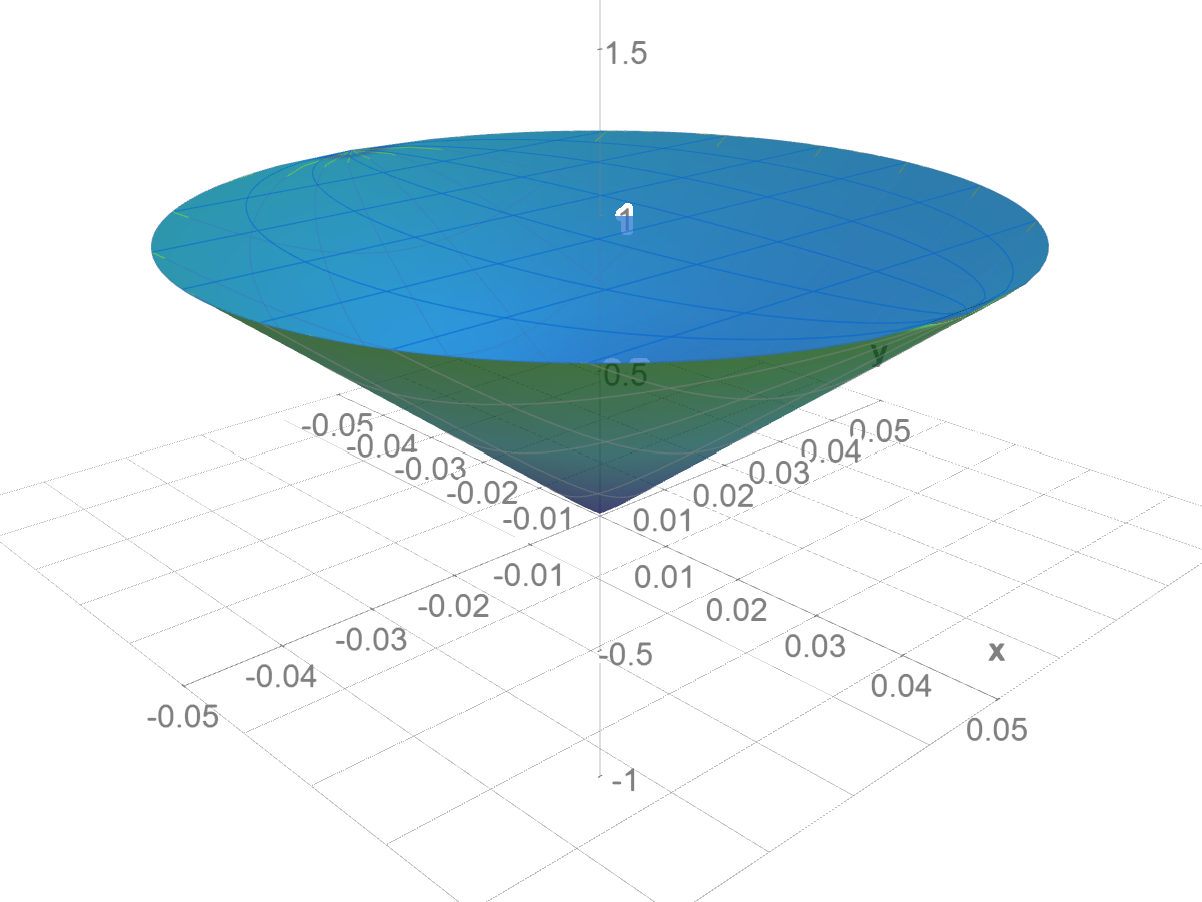
\includegraphics[scale = 0.5]{images/ex3.png}
        \caption{Sharp Cone of height 1, top radius $tan(2.5^\circ)$.}
        \label{fig:ex3}
    \end{figure}
\end{enumerate}

\section{Quadratic Tetrahedral Lagrange Basis}

When consdering 3D elements, the simplest choices include tetrahedrons and hexahedrons \cite{3d-elements}. We will be
using the unit tetrahedron, and transform it to physical element under a bijection to the same basis (isoparametric), 
and use these elements to fill our domain. \\

Table \ref{tab:shape_functions} lays out the quadratic tetrahedral lagrange basis in $(\xi_1, \xi_2, \xi_3)$ space. \\

\begin{table}[h!]
\centering
\renewcommand{\arraystretch}{1.5}
\begin{tabular}{|c|c|}
\hline
\textbf{Node Point $z_i$} & \textbf{Shape Function $\phi_i$} \\
\hline
$z_1(1,0,0)$ & $\phi_1 = \xi_1(2\xi_1 - 1)$ \\
\hline
$z_2(0,1,0)$ & $\phi_2 = \xi_2(2\xi_2 - 1)$ \\
\hline
$z_3(0,0,0)$ & $\phi_3 = (1 - \xi_1 - \xi_2 - \xi_3)(1 - 2\xi_1 - 2\xi_2 - 2\xi_3)$ \\
\hline
$z_4(0,0,1)$ & $\phi_4 = \xi_3(2\xi_3 - 1)$ \\
\hline
$z_5(\frac{1}{2},\frac{1}{2},0)$ & $\phi_5 = 4\xi_1\xi_2$ \\
\hline
$z_6(0,\frac{1}{2},0)$ & $\phi_6 = 4\xi_2(1 - \xi_1 - \xi_2 - \xi_3)$ \\
\hline
$z_7(\frac{1}{2},0,0)$ & $\phi_7 = 4\xi_1(1 - \xi_1 - \xi_2 - \xi_3)$ \\
\hline
$z_8(\frac{1}{2},0,\frac{1}{2})$ & $\phi_8 = 4\xi_1\xi_3$ \\
\hline
$z_9(0,\frac{1}{2},\frac{1}{2})$ & $\phi_9 = 4\xi_2\xi_3$ \\
\hline
$z_{10}(0,0,\frac{1}{2})$ & $\phi_{10} = 4\xi_3(1 - \xi_1 - \xi_2 - \xi_3)$ \\
\hline
\end{tabular}
\caption{Node points and corresponding shape functions}
\label{tab:shape_functions}
\end{table}

Let the unit tetrahedron be $\boldsymbol{K}$ (Figure \ref{fig:reg_tetrahedron}), and the bijective mapping
from the finite element space $(\boldsymbol{K},\boldsymbol{\mathcal{P}_2},\boldsymbol{\mathcal{N}})$ be 
$F:\boldsymbol{K} \rightarrow \mathbb{R}^3$, mapping $z_j$ to corresponding $z_j^e$ in physical domain. 
Here, $\boldsymbol{\mathcal{N}}=\{N_1, N_2, ... N_{10}\}$, with $N_j(v) = v(z_j)$. Then, the element basis 
functions over curved element $\boldsymbol{K^e} = F(\boldsymbol{K})$ is given by $\phi_j(F^{-1}(\overrightarrow{x}))$,
and let's denote the isoparametric finite element space 
$(\boldsymbol{K^e},\boldsymbol{\mathcal{P}_2^e},\boldsymbol{\mathcal{N}^e})$.

\begin{figure}[h]
    \centering
    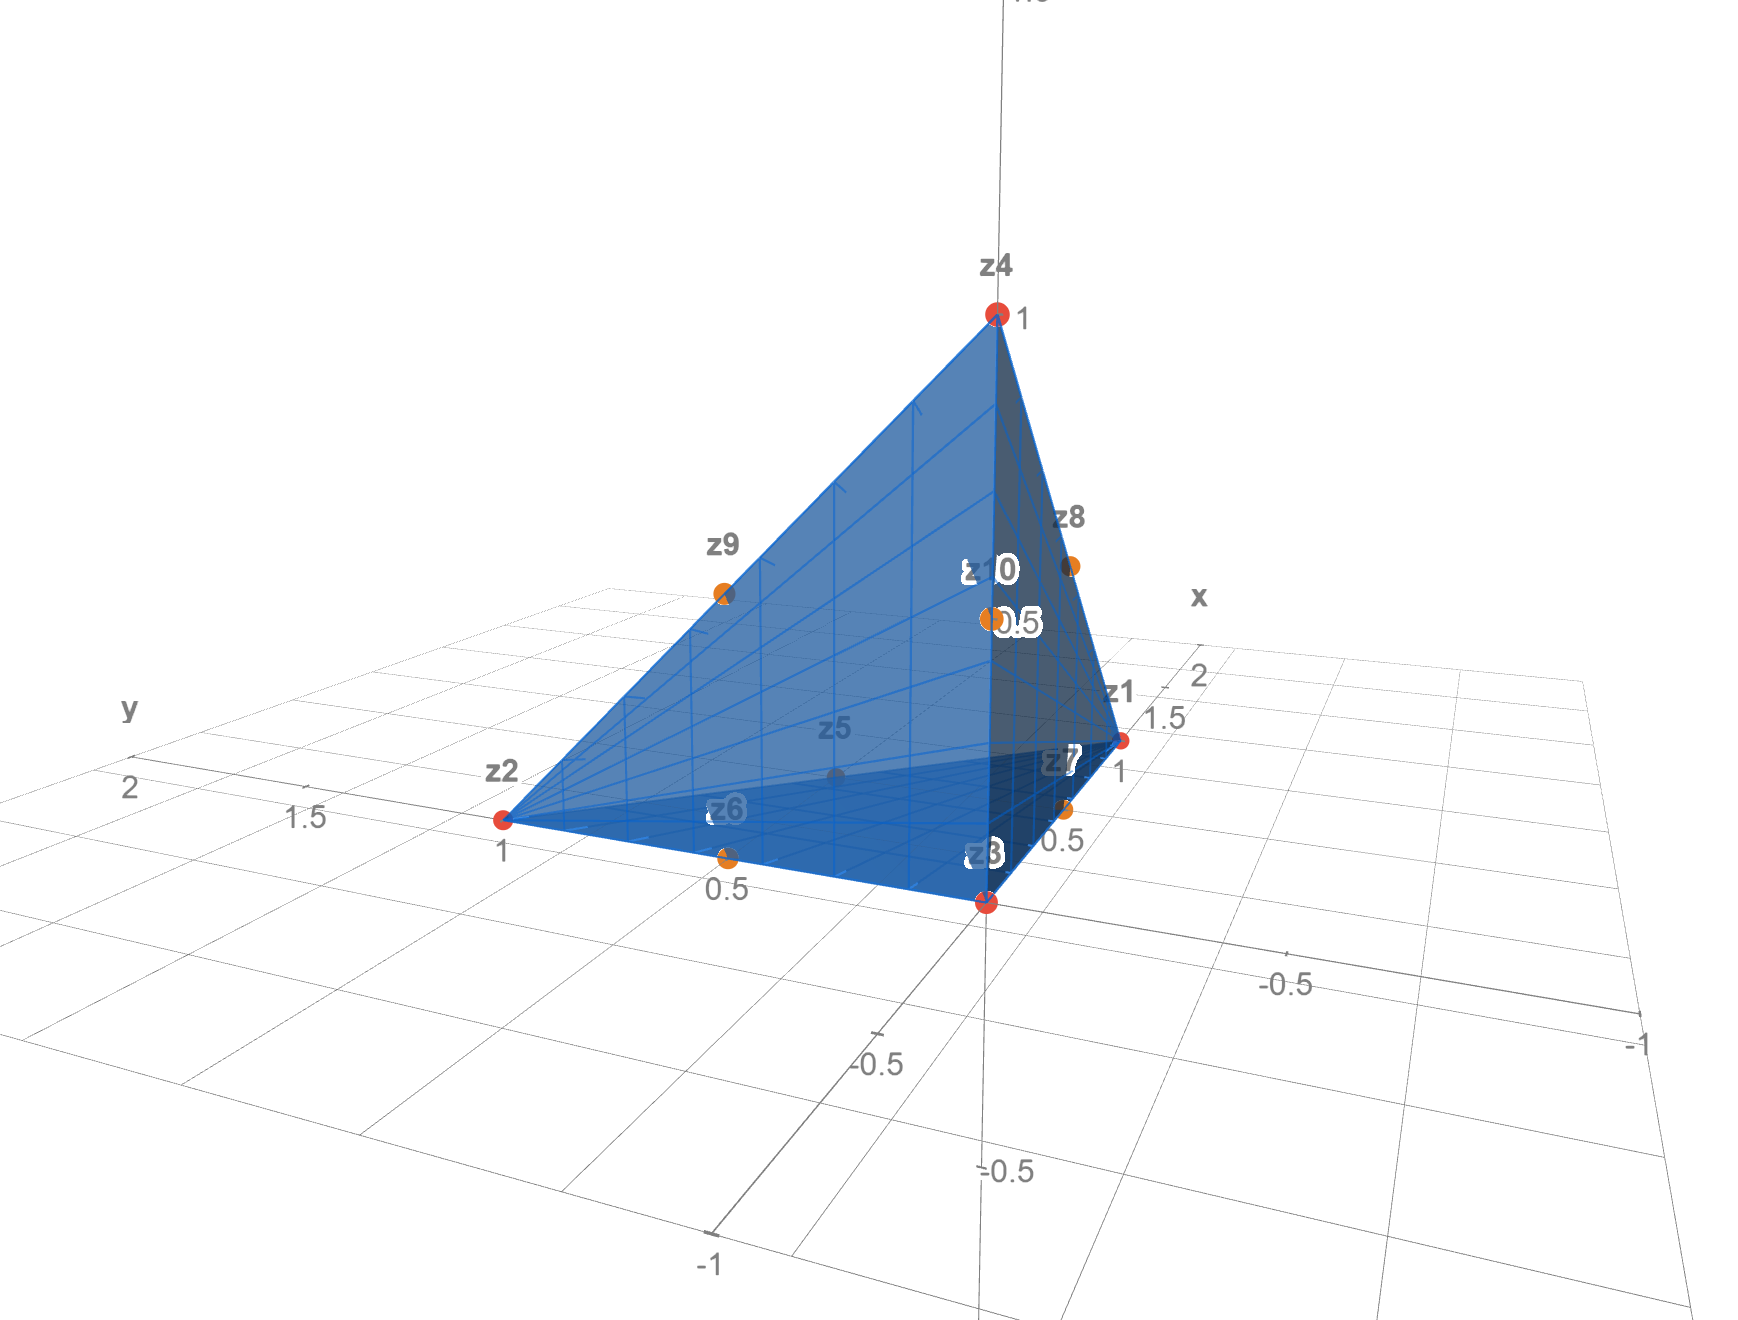
\includegraphics[scale = 0.5]{images/tetrahedron.png}
    \caption{Regular Tetrahedron.}
    \label{fig:reg_tetrahedron}
\end{figure}

\section{Weak Formulation \& Stiffness Matrix}

As seen in Homework 4, we will be relaxing the following weak formulation:

$$ \int_{\Omega} \nabla u \cdot \nabla v \, dA = \int_{\partial \Omega} \frac{\partial u}{\partial n} v \, d\ell $$

If $\gamma u = g$, note that we are considering test functions over $V = \{v \in H^1\Omega \vert \gamma v = g\}$. Therefore,
we will apply BC constraint to the linear system for the following problem explicilty:

$$ \int_{\Omega} \nabla u \cdot \nabla v \, dA = 0 $$

Equivalently, we will assemble the stiffness matrix $\boldsymbol{M}$ to solve for the vector of nodal values $u$ take, 
$\boldsymbol{U}$, with rhs as the $0$ vector, right before modifying this system with Dirichlet BC values by fixing node
values at the boundary appropriately (substituting value in other rows as required). To assemble $\boldsymbol{M}$, we need
the stiffness matrix over each element. When approximating with finite dimensional basis:

$$\boldsymbol{M}_{ij}^e = \int_{\boldsymbol{K}^e} \nabla_{\mathbf{x}} \phi_i \left( F^{-1}(\mathbf{x}) \right) \cdot \nabla_{\mathbf{x}} \phi_j \left( F^{-1}(\mathbf{x}) \right) \, d\mathbf{x}$$

Since \((x,y,z) = F(\xi_1, \xi_2, \xi_3)\), the Jacobian \(J:\boldsymbol{K} \to \mathbb{R}^{3 \times 3}\) of \(F\) is:

\[
J(\xi_1, \xi_2, \xi_3) = 
\begin{pmatrix}
\frac{\partial x}{\partial \xi_1} & \frac{\partial y}{\partial \xi_1} & \frac{\partial z}{\partial \xi_1} \\
\frac{\partial x}{\partial \xi_2} & \frac{\partial y}{\partial \xi_2} & \frac{\partial z}{\partial \xi_2} \\
\frac{\partial x}{\partial \xi_3} & \frac{\partial y}{\partial \xi_3} & \frac{\partial z}{\partial \xi_3} 
\end{pmatrix}
\]

Thus, substituting in our integral:

$$\boldsymbol{M}_{ij}^e = \int_{\boldsymbol{K}} \nabla_{\mathbf{x}} \phi_i(\mathbf{t}) \cdot \nabla_{\mathbf{x}} \phi_j(\mathbf{t}) \, |J(\mathbf{t})| \, d\mathbf{t},$$

where $\mathbf{t} = (\xi_1, \xi_2, \xi_3)$, and $\nabla_{\mathbf{x}} \phi_i(\mathbf{t})$ is evaluated by:

\[
\begin{pmatrix}
\frac{\partial}{\partial x} \phi_i \\
\frac{\partial}{\partial y} \phi_i \\
\frac{\partial}{\partial z} \phi_i
\end{pmatrix}
=
J^{-1}(\xi_1, \xi_2, \xi_3)
\begin{pmatrix}
\frac{\partial}{\partial \xi_1} \phi_i \\
\frac{\partial}{\partial \xi_2} \phi_i \\
\frac{\partial}{\partial \xi_3} \phi_i
\end{pmatrix}.
\]

We will be evaluting the integral using degree 2 quadrature rule \cite{quad-rule} for $\mathcal{O}(h^3)$ accuracy,
where $h$ is the diameter of the tetrahedron:

\[
\int_{\boldsymbol{K}} f(\mathbf{t}) \, d\mathbf{t} \approx \frac{1}{24} \left[
f\left( b, b, b \right) +
f\left( a, b, b \right) +
f\left( b, a, b \right) +
f\left( b, b, a \right)
\right], a = 0.58541020, b = 0.13819660 .
\]

\section{Mesh Generation}

\textit{gmsh} has a rich API to create and optimize meshes for objects in 1 to 3 domensional spaces. We select
Frontal-Delaunay mesh algorithm for surfaces in our 3D objects, and Frontal 3D mesh algorithm, running on top of
OpenCASCADE CAD kernel. Frontal is necessary to generate quadratic order tetrahedral mesh for our volumetric 
objects. We further generate meshes for MSFs from 1/2 to 1/8. Figures \ref{fig:gmsh_sph}, \ref{fig:gmsh_cyl} \&
\ref{fig:gmsh_con} provide a view of generated mesh for MSF = 0.5 . 

\begin{figure}[h]
    \centering
    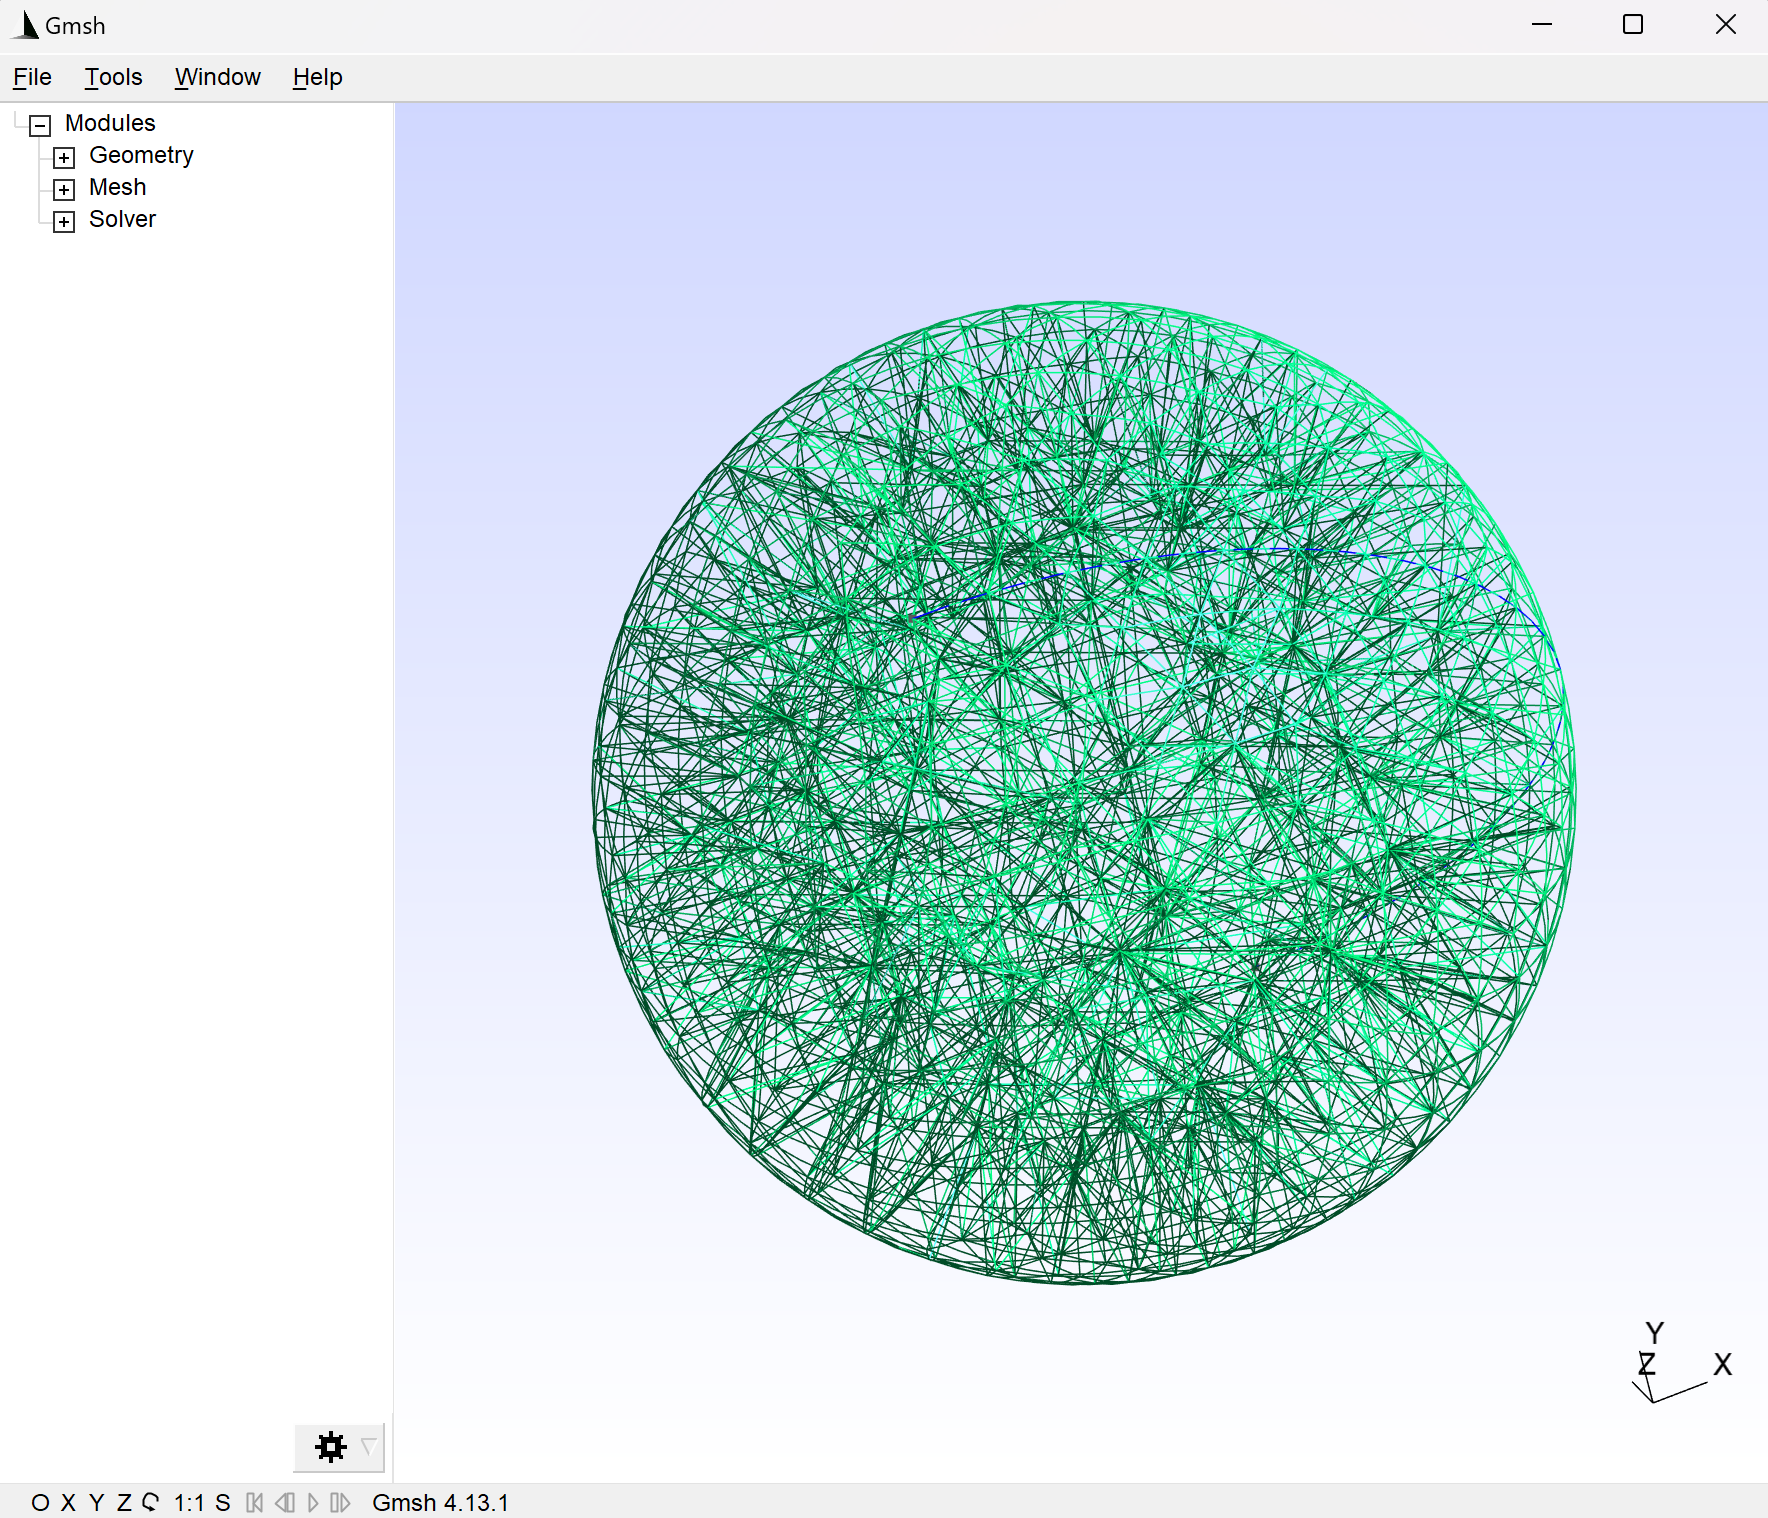
\includegraphics[scale = 0.4]{images/gmsh_sphere.png}
    \caption{Mesh for sphere from case 1, $MSF = 0.5$ .}
    \label{fig:gmsh_sph}
\end{figure}

\begin{figure}[h]
    \centering
    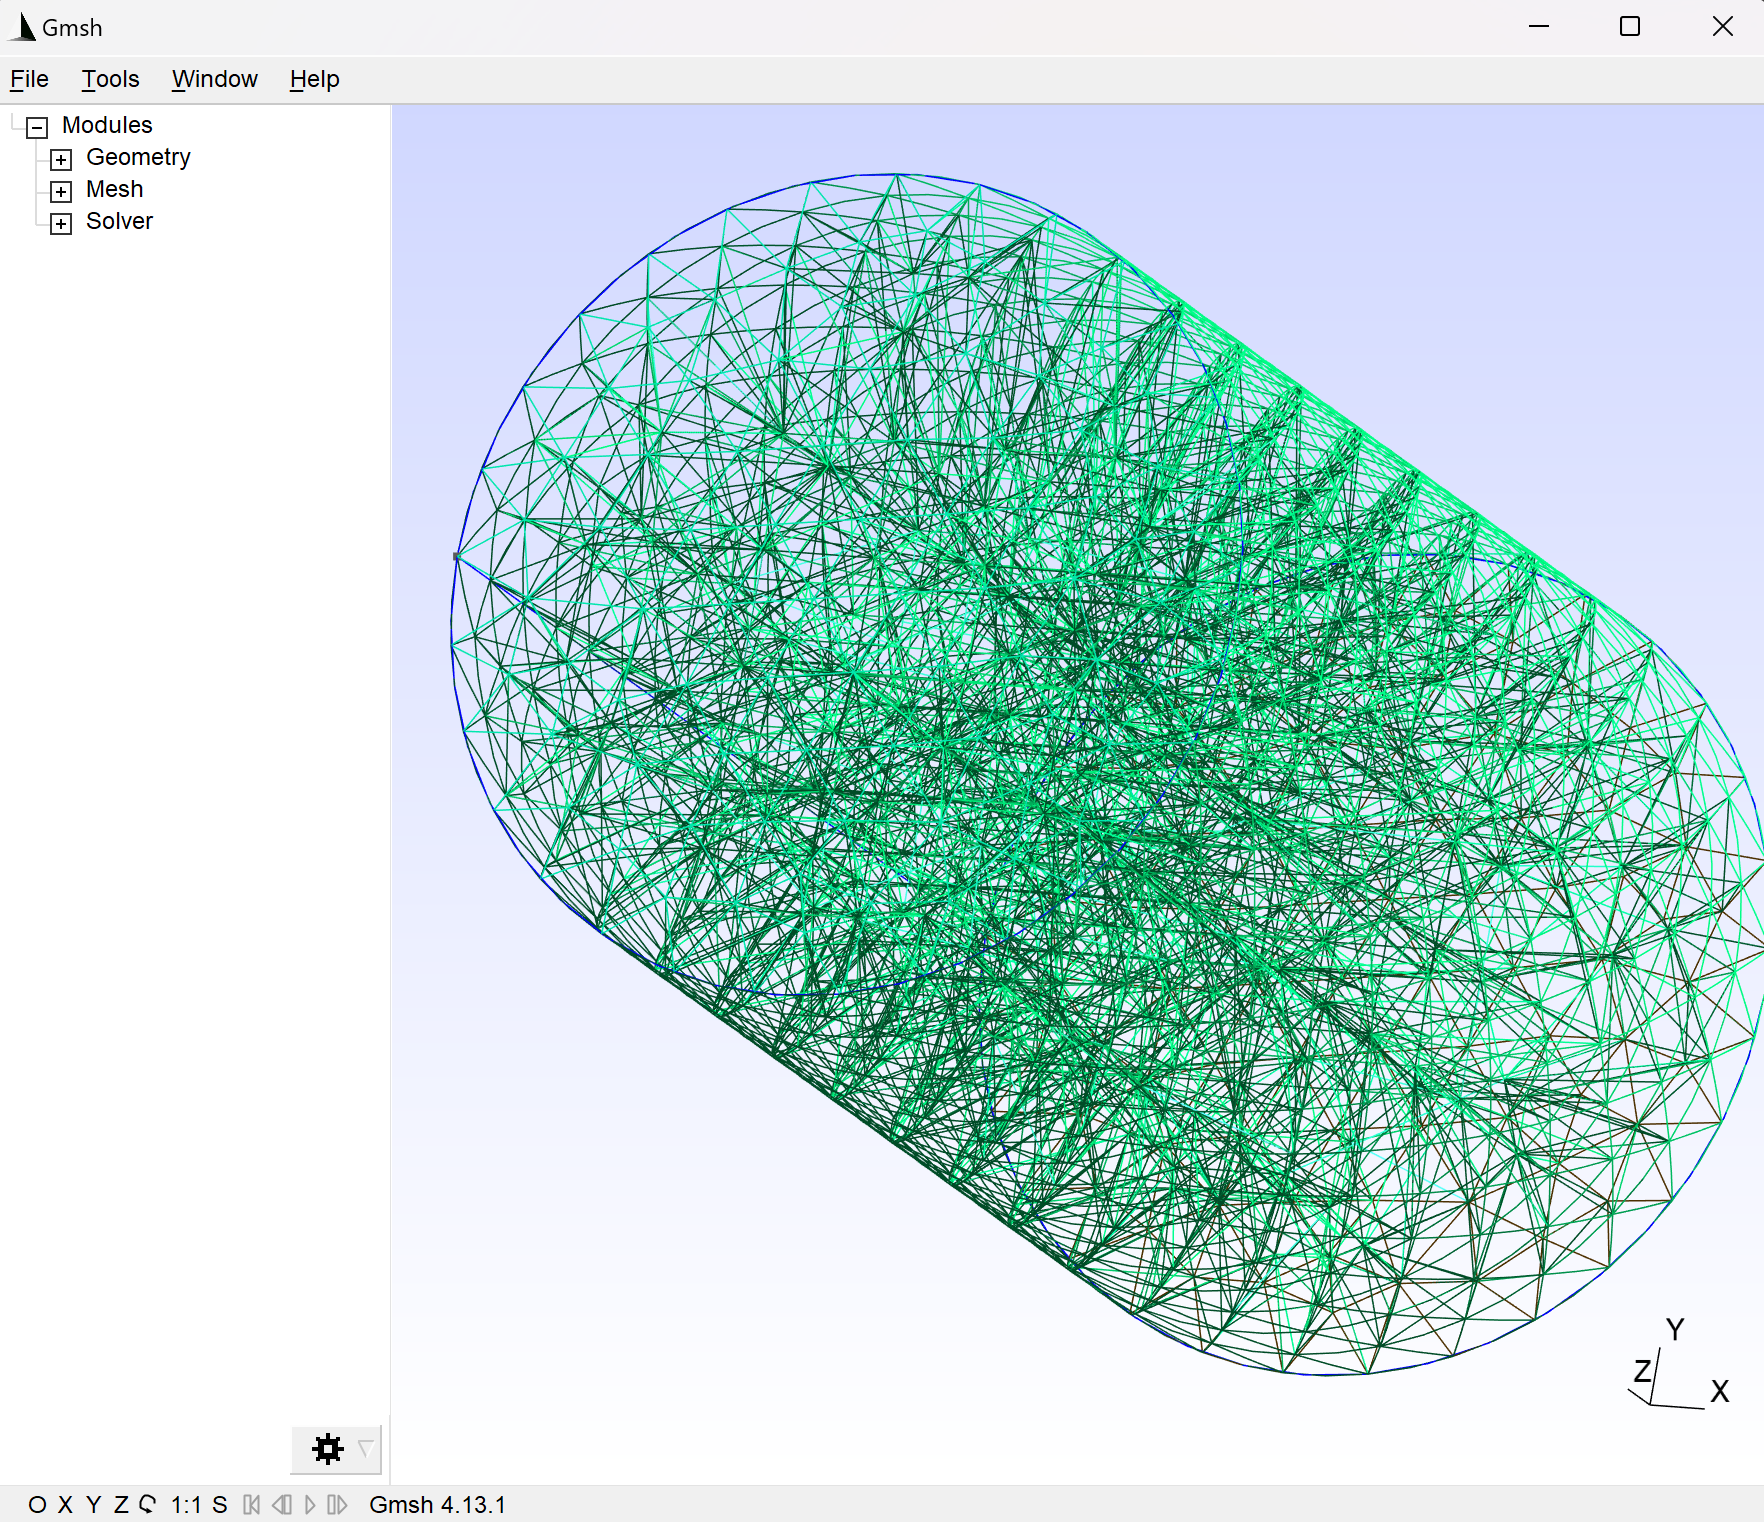
\includegraphics[scale = 0.4]{images/gmsh_cylinder.png}
    \caption{Mesh for cylinder from case 2, $MSF = 0.5$ .}
    \label{fig:gmsh_cyl}
\end{figure}

\begin{figure}[h]
    \centering
    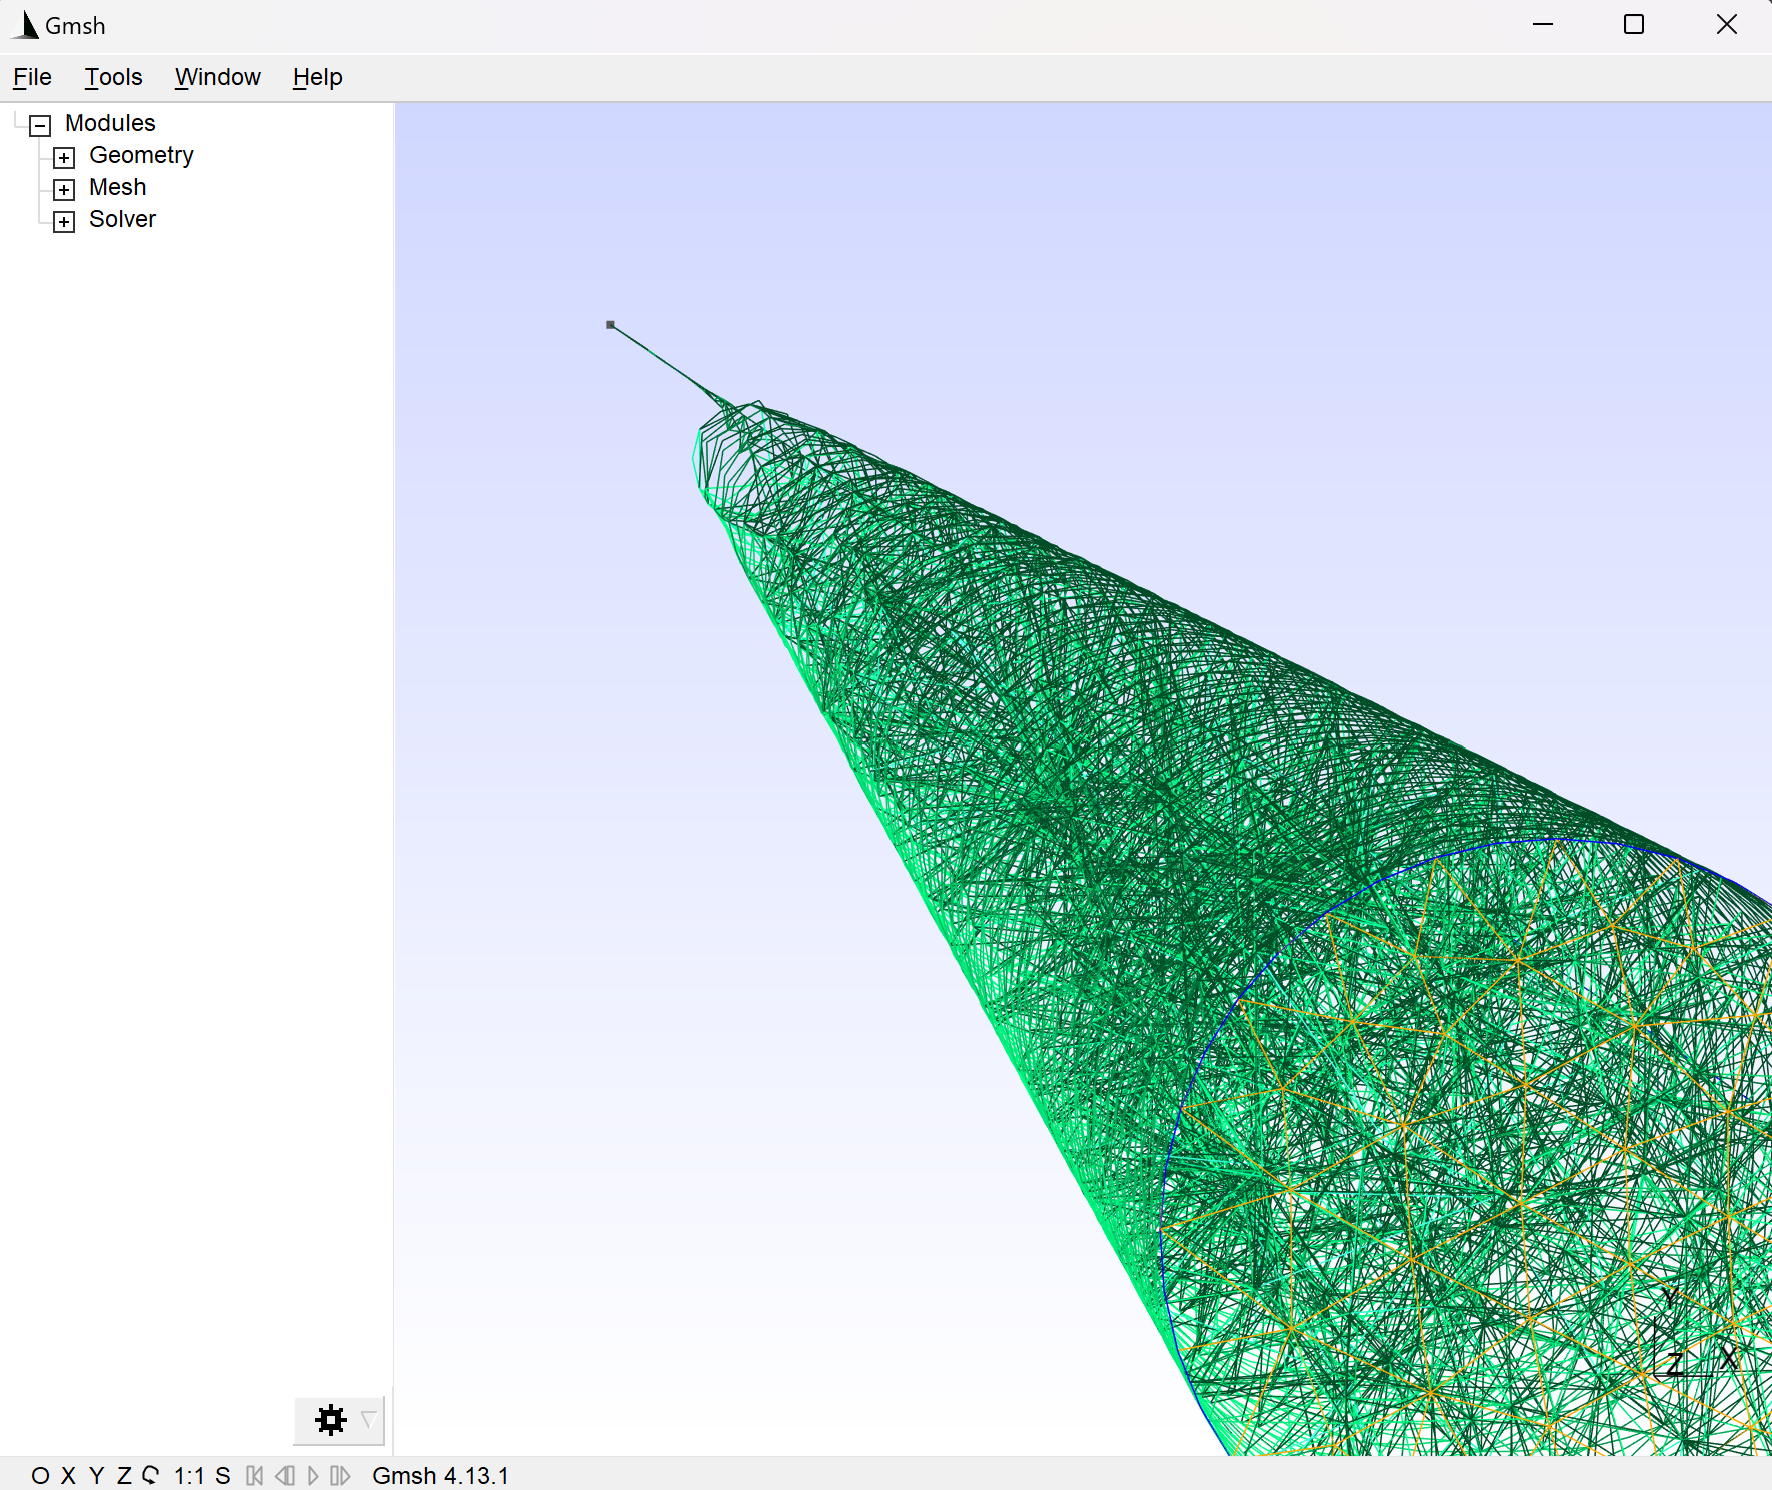
\includegraphics[scale = 0.4]{images/gmsh_cone_smooth.png}
    \caption{Mesh for cone from case 3, $MSF = 0.29$ .}
    \label{fig:gmsh_con}
\end{figure}

\textit{gmsh} also includes the ability to smooth corners, having an option which stores the number of mesh smoothening
iterations. This can be particularly helpful when things misbehave around the boundary, specifically edges that don't form
90 degrees, causing singularities in solution. Thus, for case 3, given the apex of a sharp cone, we test the effect of 
smoothening by comparing unsmoothened mesh based solution and 10 iterations worth of smoothening based mesh solution.

\section{Results}

We calculate computed solution errors by:

\[
    \varepsilon^h_u = \max_i \left| u_i^h - u(\mathbf{x}_i) \right|, \mathbf{x}_i \text{ node}.
\]

Since $g$, the Dirichlet BC, is harmonic, $u = g$. Thus, we easily and quickly find max error using above formula.
Below are observations for the different case studies:

\begin{itemize}
    \item In case 1, we reach numerical limits on computation as we reach $MSF=0.3$, performing worse than $MSF=0.5$;
    The effect of computational limits is reached faster due to the pure curved surface of the case, a sphere, since generating
    mesh for curvature is generally much harder.
    \item We couldn't compute solution for $MSF = 1/8$ in case 2, given the large volume of the cylinder implying large number of
    finite elements. We observe relatively slower improvements with finer mish otherwise, but not surprising given the majority
    curved surface of the cylinder.
    \item In case 3, we observe the benefits of smoothening, an improvement of $\approx 10^{-5}$. Note, we can potentially get
    worse solution if we over-smoothen sharp edges which are not 90 degrees!
\end{itemize}

\begin{table}[h!]
    \centering
    \renewcommand{\arraystretch}{1.2}
    \begin{tabular}{lccc}
    \hline
    \textbf{Geometry} & \textbf{MSF} & \textbf{$h_{\max}$} & \textbf{$\varepsilon_u^h$} \\
    \hline
    \multirow{3}{*}{Case 1: Sphere} 
      & 0.50 & 3.0870 & 0.0346 \\
      & 0.35 & 1.9430 & 0.0331 \\
      & 0.30 & 1.8449 & 0.0348 \\
    \hline
    \multirow{2}{*}{Case 2: Cylinder} 
      & 0.50 & 1.9032 & 0.0219 \\
      & 0.25 & 0.8747 & 0.0185 \\
    \hline
    \multirow{2}{*}{Case 3: Cone} 
      & 0.29 (no-smooth) & 0.0415 & 1.7204e-04 \\
      & 0.29 (smooth)    & 0.0402 & 1.5950e-04 \\
    \hline
    \end{tabular}
    \caption{Computed solution errors for cases 1,2 and 3.}
\end{table}

\newpage

\bibliographystyle{plain}
\bibliography{refs}
\end{document}